%
% TikZ code to draw a complete k-partite graph
%
\documentclass[tikz]{standalone}

\begin{document}

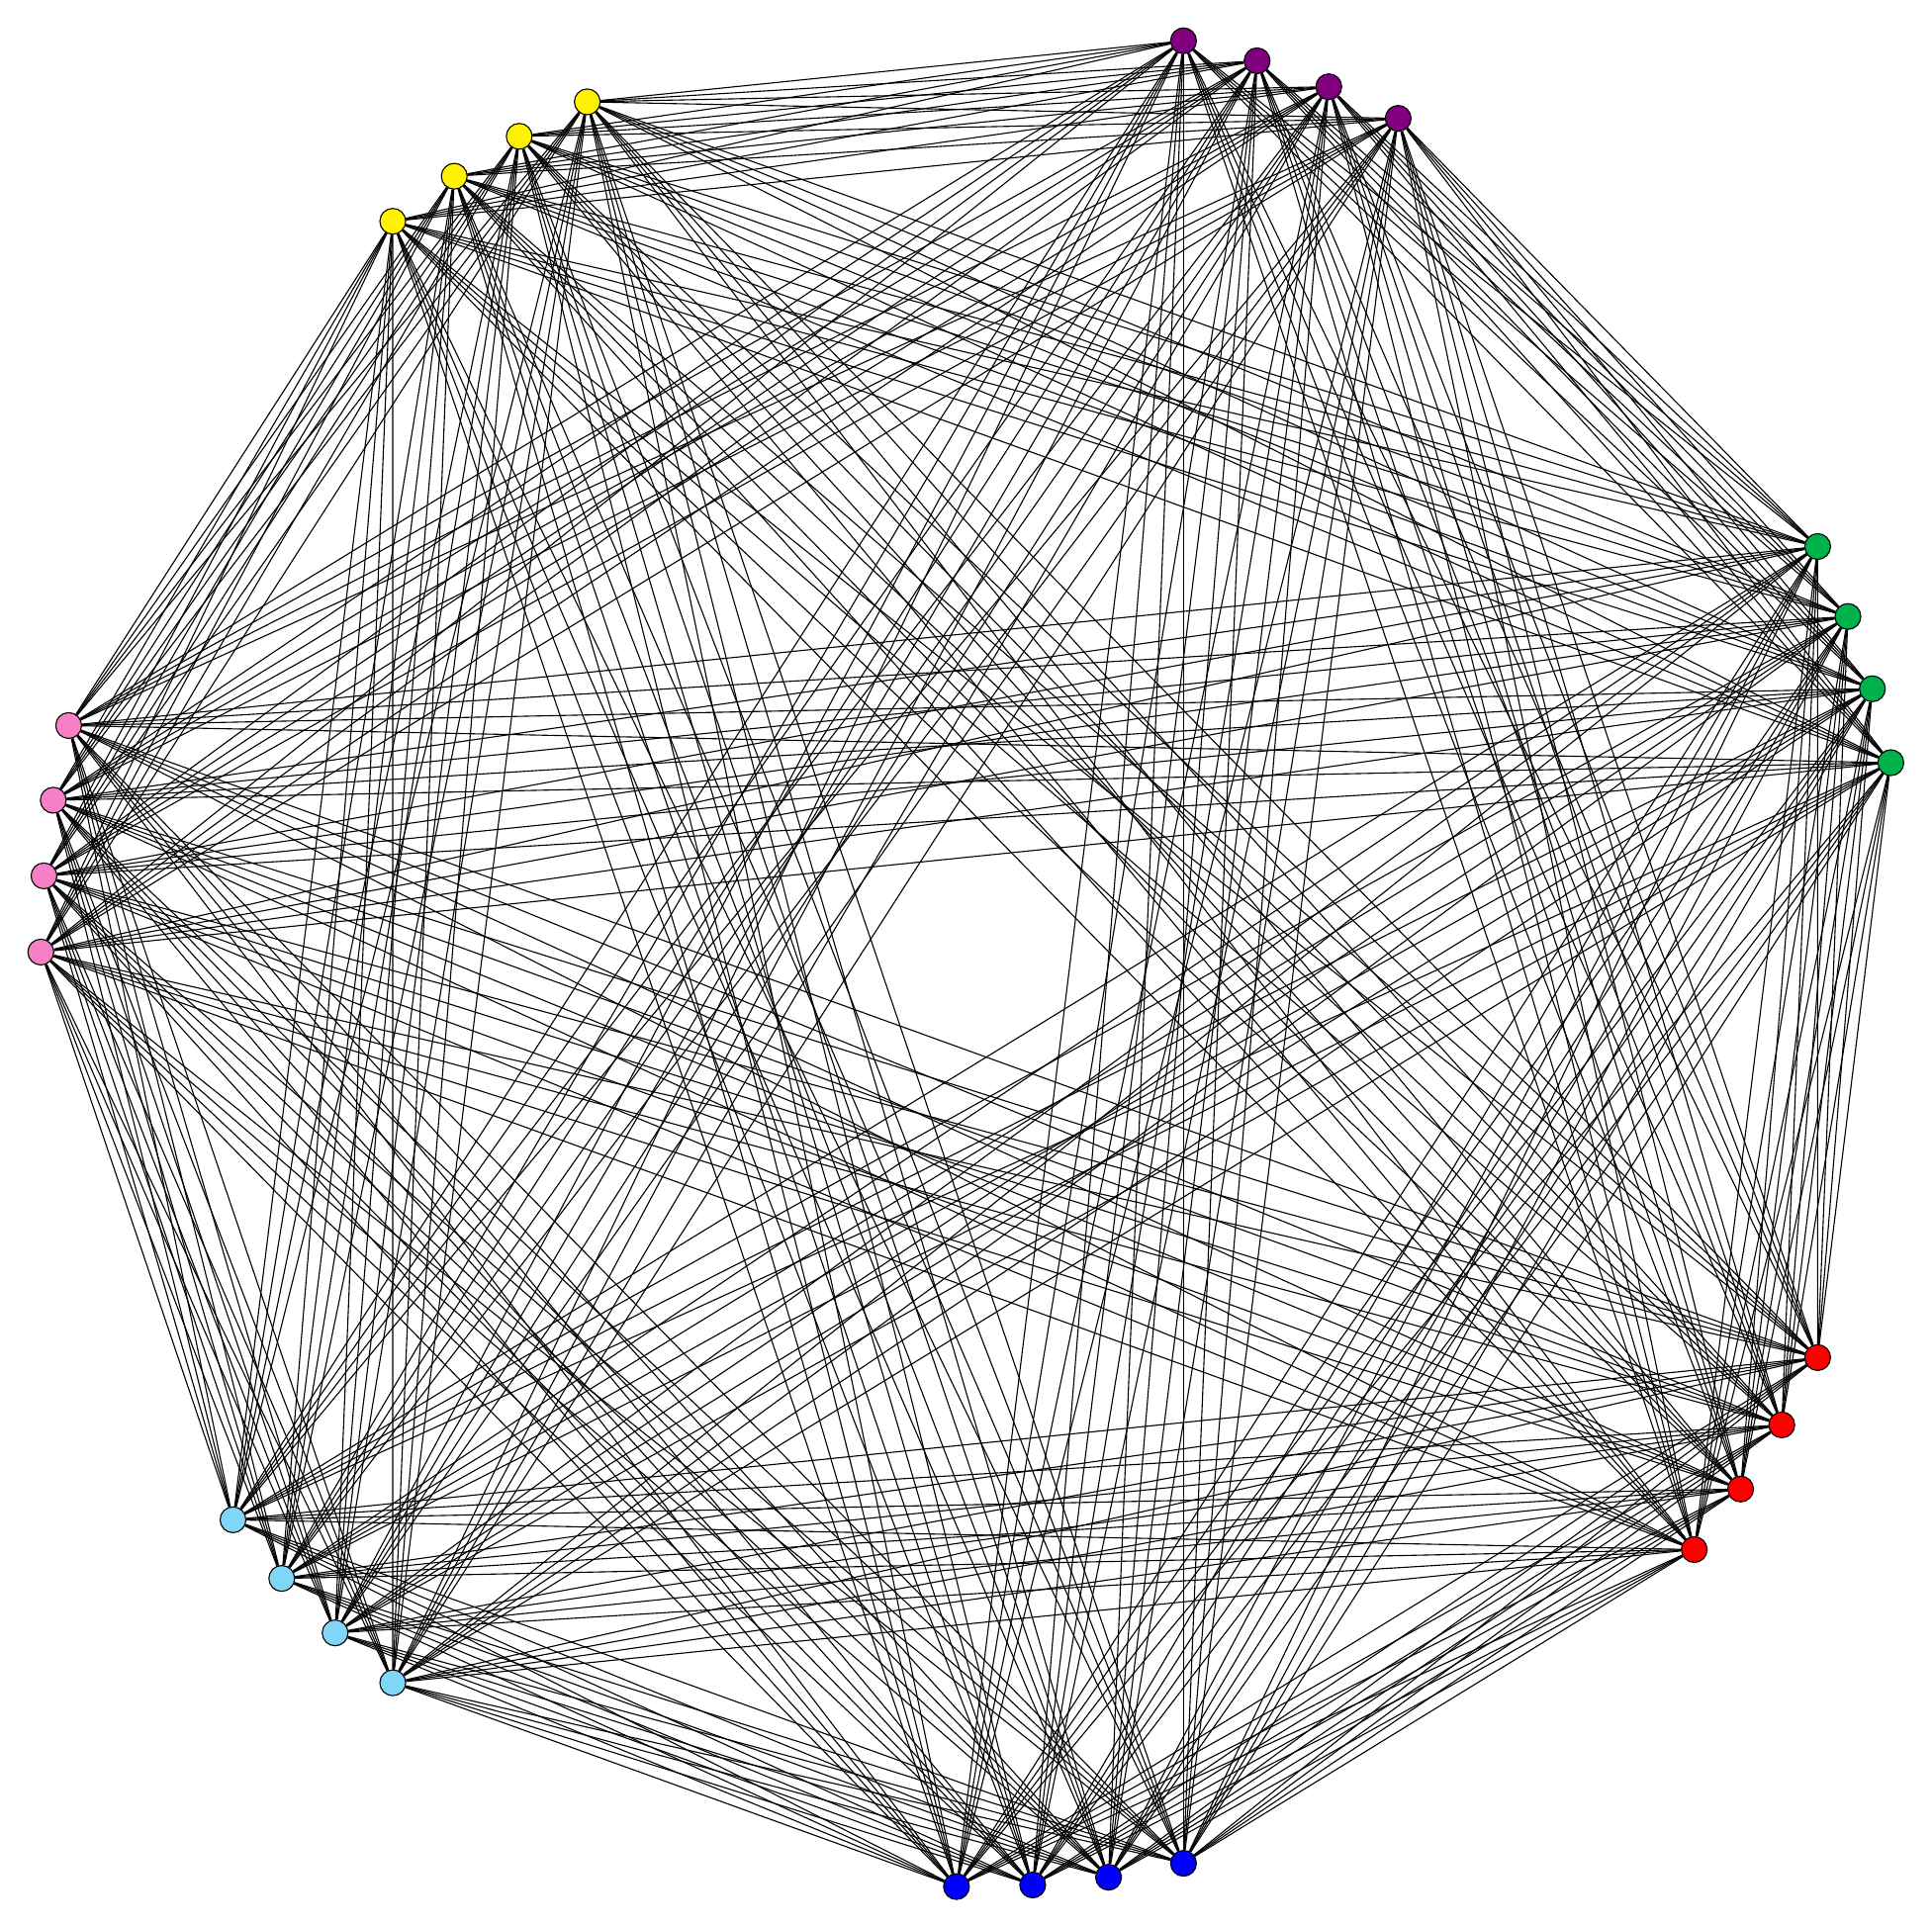
\begin{tikzpicture}

	\def\n{4}				% number of nodes in each part
	\def\k{7}				% number of parts 
	
	%drawing parameters
	\def\r{12}				% radius of the circle
	\def\spacing{7}		% amount of spacing between the parts
	\def\bend{0}				% amount of bending of the edges
	\def\coloring{1}		% Boolean value telling to show (or not) the \k-coloring (if set to 1 then \k must be smaller than 8 or otherwise make the array \mycolors longer)
	\def\showclique{0}	% Boolean value telling if we want to show a \k-clique
	\def\hidepart{0}		% Remove one of the parts of the \k-partite (0 to show all the parts)
	
	\newcommand{\mycolors}{{"white", "blue", "red", "green!70!blue", "violet", "yellow", "magenta!50!white", "cyan!50!white", "lime!90!red"}} %array of colors for the \k-coloring, make longer for k\ge 9
	
	\foreach \i in {1,...,\k}{% draw the vertices
		\ifnum\coloring=0
			\pgfmathsetmacro\color{\mycolors[0]}%default color of vertices
		\else
			\pgfmathsetmacro\color{\mycolors[\i]}% set the colors into groups according to \mycolors 
		\fi
		\foreach \j in {1,...,\n}{
			\pgfmathparse{360/(\k*(\n+\spacing))*(\i*(\n+\spacing)+\j+\spacing)}%how the arithmetic is written here is *relevant*
			\ifnum\i=\hidepart
			\else
				\draw (\pgfmathresult : -\r) node[draw=black, circle, fill=\color] (\i\j){};
			\fi
		}
	}
	
	\foreach \x in {1,...,\k}{% draw edges
		\foreach \y in {\x,..., \k}{
			\foreach \i in {1,...,\n}{
				\foreach \j in {1,..., \n}{
					\pgfmathparse{(\y>\x) && (\y!=\hidepart) &&(\x!=\hidepart)}
					\ifnum\pgfmathresult=1
						\draw (\x\i) to [bend right=\bend] (\y\j);
					\fi
				}
			}
			\ifnum\showclique=1
				\draw[ultra thick, red] (\x1) to [bend right=\bend] (\y1); % to highlight the clique
			\fi
		}
	}
	
\end{tikzpicture}	

\end{document}